\subsection{Application description}
GHio-Ca (Giving Hashtags In Order To Classify Automatically) is an Android
application that gives to a user the possibility to make image recognition on
her pictures. This application embed some camera features in order to make
possible to take a photo and recognize it directly, but it also allows to pick
a picture from the saved ones and launch the classifying process on it.
GHio-Ca is specifically designed to recognize objects and text: the only
limitation is that the user has to choose it before starting the
recognition process from the hamburger menu placed in the main activity.
The overall application is mainly composed by four activities:
\begin{itemize}
  \item splash activity: this view is needed in order to gain from the user
    the necessary permissions (network access, camera access, access to
    the storage);
    \begin{figure}[h]
        \centering
        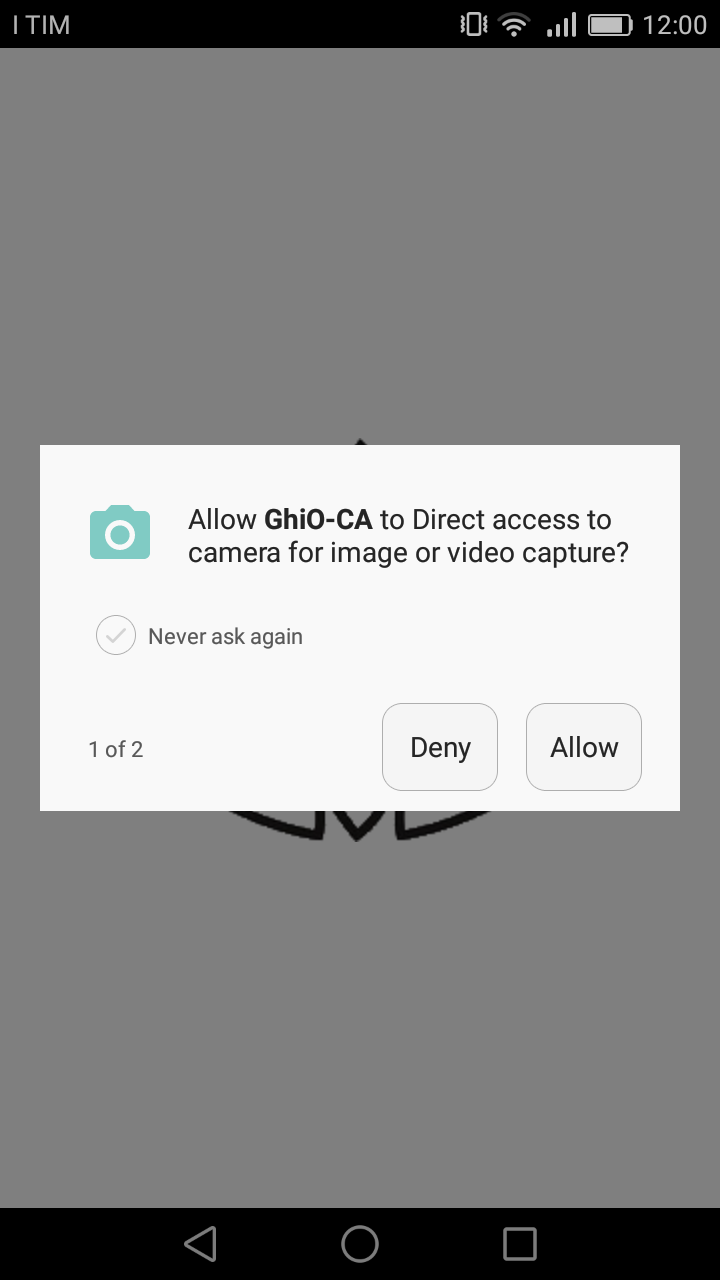
\includegraphics[width=0.18\textwidth]{../img/splash}
        \caption{Screen-shot of the splash activity, when authorization are 
                 required}
        \label{fig:splash}
    \end{figure}
  \item camera preview activity: this one displays the user a camera
    interface, with the possibility to take photos, turn off the flash, switch
    to frontal camera (if present) and to access to the gallery in order to
    pick a file instead of taking a picture. In the top left corner is present
    the hamburger menu: it allows user to choose the size of picture taken,
    it reminds the user to turn on the Wi-Fi sensor on every access and it
    allows to switch from the image recognition functionality to the
    character optical recognition feature and vice-versa;
    \begin{figure}[h]
        \centering
        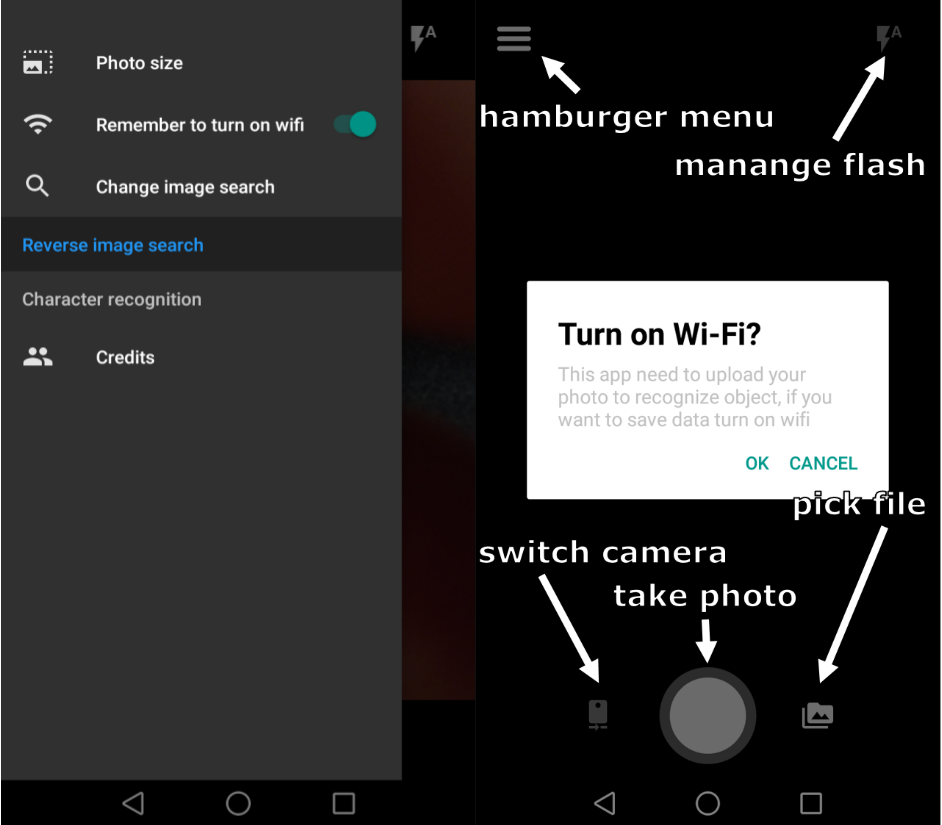
\includegraphics[width=0.30\textwidth]{../img/main_activity}
        \caption{Screen-shots of the main activity, with and without open 
                 hamburger menu}
        \label{fig:splash}
    \end{figure}
  \item results activities: these are two different activities depending on
    the type of image recognition chosen.
    \begin{itemize}
     \item If the ``reverse image search'' functionality is enabled then the
result activity will contain a photo thumbnail, a description and a list of
tags. Any tag can be deselected by the user if it doesn't fit the image.
    \begin{figure}[h]
        \centering
        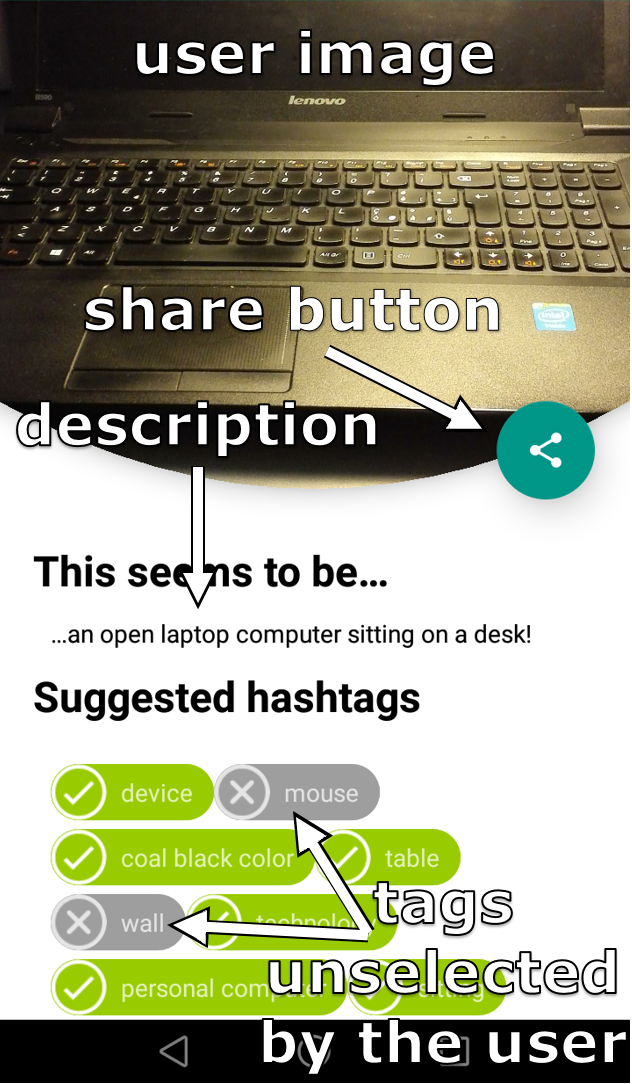
\includegraphics[width=0.18\textwidth]{../img/image_result_activity}
        \caption{Screen-shots of the result activity for image recognition}
        \label{fig:splash}
    \end{figure}
     \item With ``optical character recognition'' on, instead, the result
activity will display the photographed text and its OCR translation. The user
will be able to pick another translation from a drop down menu.
    \end{itemize}
\end{itemize}

\subsection{libris}
Libris(Library Reverse Image Search) is a library that we develop in order to 
simply the image recognition process. This library has the job to make call to 
the different services that we used in order to fulfill the image or character 
recognition, defining an interface for the results.

All the requests return a response in JSON format, that will be parsed and the 
more informative fields are embedded in a object, different for every service, 
that will be returned. 

If some error occur during the request an IOException will be thrown.

For image recognition libris gives the possibility to use: Azure, Watson, Immaga 
and Google Reverse Image Search. In order to provide the latter service we 
programmatically search on Google the image, catching the beast result returned.

For Character recognition libris give the chance to utilize: Watson OCR(still in 
beta), Azure OCR and FreeOCRSpace.

\subsection{CameraFragment}
CameraFragment is a library that simplify the camera using in Android. It's 
open source and freely available on Github [TODO insert link]. Because of some
issues in the library, mainly caused by the wrong management of Android Camera1 
and Camera2, and because the usage of some parts of that library differed from 
the one expected in GHio-Ca, we decided to modify that project, changing those 
parts that were not functional to the project.

\subsection{Architecture}
GHio-Ca is principally composed by two layers: (i) the one that have to manage
network connectivity, uploading photos to the server and making requests to 
different services in order to make the image recognition or the translation of 
certain pieces of text, and (ii) the camera layer, that manages the photo 
capturing process and saving. 

These two layers are maintained as loose coupled as possible in order to make 
easy to change services used without making important changes to the overall 
application or changing the process of photo taking, without modify the 
networking layer.

%TODO
%	-add a UML of the application architecture at really high level
%		   NETWORK
%		
%		|-----------|		|-----------|
%		| LISTENERS |------>|	PHOTO	|
%		| ASYNCTASK |<------|			|
%		|-----------|		|-----------|

In order to make network calls for image recognizing we implemented a utility 
class that offers the possibility to create AsyncTasks, different for every 
service, that will be executed on a thread pool (in order to make possible to 
fulfill more tasks at same time). To each of those AsyncTask it must be associate 
a listener in order to collect all the results of the search. Practically, 
classes that implement the interface Listener expose methods 'onStart()', 
'onFailure()' and 'onSuccess()', that will be called from the AsyncTask. The 
first one is called in 'onPreExecute()' method, 'onFailure()' is invoked in 
'onPostExecute()' if during the 'doInBackground()' method some error occurred 
and, the latter one is called if the 'doInBackground()' method is executed 
without any issue, during 'onPostExecute()'.

Thanks to the possibility of detect image recognition process failure and since 
we use more services, we have implemented some robustness feature in our 
application, making it returning an error to the user only if all services fails. 
The scenario where, even if the application could start the image recognition 
process but it could not be able to finish it, could still occurs, for example 
caused by a network fault.

If no errors occurs, we decided to skim result based on the probability that a 
word (or group of words) could be correlated to the user picture. So, if the 
service allowed us, we only take result that have an high probability, fixing the 
threshold to 70\% (we have fixed it empirically). If the service provides no 
probability, it generally divide results in two sets based on the fact that a 
certain word could be more or less correlated to the picture. In that case we 
only present to the user only the more correlated results.

This layer not only have the job to search the image but it have to offer the 
possibility to upload the image that must be recognized. Because of limitation 
of some services and in order to save user data we decided to upload the 
application to a server and pass to the different services the URL to which the 
image is accessible. With this approach we allow users to save data because you 
only need to upload the photo once and profit by the URL to make the recognition 
with more services.